%%%%%%%%%%%%%%%%%%%%%%%%%%%%%%%%%%%%%%%%%
% Short Sectioned Assignment
% LaTeX Template
% Version 1.0 (5/5/12)
%
% This template has been downloaded from:
% http://www.LaTeXTemplates.com
%
% Original author:
% Frits Wenneker (http://www.howtotex.com)
%
% License:
% CC BY-NC-SA 3.0 (http://creativecommons.org/licenses/by-nc-sa/3.0/)
%
%%%%%%%%%%%%%%%%%%%%%%%%%%%%%%%%%%%%%%%%%

%----------------------------------------------------------------------------------------
%	PACKAGES AND OTHER DOCUMENT CONFIGURATIONS
%----------------------------------------------------------------------------------------

\documentclass[paper=a4, fontsize=11pt]{scrartcl} % A4 paper and 11pt font size

\usepackage[T1]{fontenc} % Use 8-bit encoding that has 256 glyphs
\usepackage[english]{babel} % English language/hyphenation
\usepackage{amsmath,amsfonts,amsthm} % Math packages
\usepackage{listings}
\usepackage{lipsum} % Used for inserting dummy 'Lorem ipsum' text into the template
\usepackage{tabularx} % in the preamble

\usepackage{siunitx}
\sisetup{output-exponent-marker=\ensuremath{\mathrm{e}}}

\usepackage{graphicx}
\graphicspath{{./}}

\usepackage{amsmath}
\DeclareMathOperator*{\argmax}{arg\,max}
\DeclareMathOperator*{\argmin}{arg\,min}
\DeclareMathOperator\erf{erf}

% \usepackage{sectsty} % Allows customizing section commands
% \allsectionsfont{\centering \normalfont\scshape} % Make all sections centered, the default font and small caps

% \usepackage{fancyhdr} % Custom headers and footers
% \pagestyle{fancyplain} % Makes all pages in the document conform to the custom headers and footers
% \fancyhead{} % No page header - if you want one, create it in the same way as the footers below
% \fancyfoot[L]{} % Empty left footer
% \fancyfoot[C]{} % Empty center footer
% \fancyfoot[R]{\thepage} % Page numbering for right footer
% \renewcommand{\headrulewidth}{0pt} % Remove header underlines
% \renewcommand{\footrulewidth}{0pt} % Remove footer underlines

\renewcommand{\thesubsection}{\thesection.\alph{subsection}} % Designate subsections by alphas

\setlength{\headheight}{13.6pt} % Customize the height of the header

\setlength\parindent{0pt} % Removes all indentation from paragraphs - comment this line for an assignment with lots of text

%----------------------------------------------------------------------------------------
%	TITLE SECTION
%----------------------------------------------------------------------------------------

\newcommand{\horrule}[1]{\rule{\linewidth}{#1}} % Create horizontal rule command with 1 argument of height

\title{	
\normalfont \normalsize 
\textsc{Michigan State University} \\ [25pt] % Your university, school and/or department name(s)
\horrule{0.5pt} \\[0.4cm] % Thin top horizontal rule
\huge Philadelphia Phillies R \& D Questionnaire \\ % The assignment title
\horrule{2pt} \\[0.5cm] % Thick bottom horizontal rule
}

\author{Kirby Hermansen} % Your name

\date{\normalsize\today} % Today's date or a custom date

\begin{document}

\maketitle % Print the title

%----------------------------------------------------------------------------------------
%	PROBLEM 1
%----------------------------------------------------------------------------------------

\numberwithin{equation}{subsection}

\section{Outfielder Proposal}

The issue at the heart of this question is unknown. Given the outfield coach's report, Player X could have any number of issues with his performance, which may or may not be treatable with drills or targeted research. Having said this, there are several potential problems to troubleshoot and help us and other members of the organization better understand the situation. Here, I will lay out my proposed troubleshooting methodology, as well as the indicative data and potential solutions. Simplified results are shown in Tab. \ref{tab:of}


\subsection{Fielding Evaluation} \label{sub:field}

Given the coach's expressed concerns of Player X---``too many errors'' and ``failing to get to some balls''---I would expect the main issue would be in Player X's performance fielding hit balls.

\subsubsection{Fielding Positioning} \label{subsub:fieldpos}

All hitters have a spray chart showing the outcomes of their at-bats \cite{baseballsavant}. It would be useful to compare that spray chart to the outfielder's original positioning for each case and calculate the difference. For the case of Player X, it may be that, when compared with the average of other fielders, he is actually being asked to cover greater distances to make plays, which may either be due to poor luck (in which case the discrepancy would go away under a larger sample size) or poor positioning by the coaches.  



\subsubsection{Fielding Range} \label{subsub:fieldrange}

As in Sec. \ref{subsub:fieldpos}, calculating the distance that Player X has to cover on his plays gives us an idea of his fielding range. Moreover, it is possible to highlight the plays where he is underperforming and dig deeper into what may have caused this. For instance, there may be plays where he failed to complete an out despite not having to cover as much ground. These likely will be cases where the launch angle and/or exit velocity off the bat is much more difficult to field quickly (a hard line drive) compared to a lazy fly ball. If there are in fact plays where he is not converting lazy fly balls into outs, these are incredibly important to identify and resolve. Regardless, his actions on either set of plays can give an insight into what may be causing his fielding issues. 

Potential solutions to these problems include better training on first steps, and honing in on how to read particular types of batted balls.

\subsubsection{Ballpark Features}

Finally, all ballparks are inherently different, and this has particular impact on an outfielder's play. It is important to verify that this is not the case for Player X. In order to do so, I would compare the metrics disccussed in Sec \ref{subsub:fieldpos} and \ref{subsub:fieldrange} in his performance at home or away and see if there is a notable difference. If so, more practice with the features of that ballpark would be in order.

\subsection{Arm Evaluation} \label{sub:arm}

As the coach specifically mentions how good Player X's arm is, I get the feeling that both his accuracy and arm strength are not major issues but they are still worth addressing.

\subsubsection{Accuracy}

First thing to consider is to confirm that the player knows where he should be throwing the ball under every situation. If he is hesitating or unsure where the throw should go, that doubt may already be enough to cause the throw to miss the mark. This can be evaluated by seeing if there is any consistency to the types of plays or the particular target on the field when Player X has made a throwing error (it also would be worth it for the outfield coach to quiz Player X on a few situations to be sure). 
\\

Possible remedies include studying the situational aspect and practicing making the target throws.

\subsubsection{Arm Strength}

Since the two concerns the coach highlights are ``errors'' and ``failing to get to some balls'' I suspect that arm strength is not a major concern for Player X. However, it is worth it to quickly confirm that he is not ``overthrowing'' on throws. Here it would be useful to check arm angles, release points, and exit velocity from Player X's throws to confirm they fit within comparable player's ranges.
\subsection{Results}

The different metrics discussed in Sec \ref{sub:arm} and \ref{sub:field} are by no means an exhaustive list of the potential hazards which are hampering Player X's performance, but would provide a decent start at troubleshooting the problems. 

\begin{table}
\begin{center}
\begin{tabularx}{\textwidth}{ |X|X|X| }
 \hline
 Problem & Data to Diagnose & Solution \\ [0.5ex] 
 \hline
 \hline
 Fielding Positioning & difference of spray chart and fielding position & more analytics into fielding to position Player X properly\\
\hline
 Fielding Range & comparison of fielding position with batted ball statistics & better training on first steps, and honing in on how to read particular types of batted balls \\
\hline
 Ballpark Features & comparison of home/away statistics & more training with particular elements of the ballpark\\
\hline
 Arm Accuracy & look at types of plays where throwing errors occur & practice and situational training\\
\hline
 Arm Strength & arm angles, release points, exit velocity & arm strength training \\

 \hline
\end{tabularx} \label{tab:of}
\end{center}
\caption{Summary of proposed problems, data, and solutions. See text for details}
\end{table}
\section{ OBP Predictor }

\subsection{Methodology}

As is typical with baseball datasets, the primary issue I encountered is dealing with incomplete or inconsistent data points for each player listed. Many players have several years where they either did not play or no data is available. This makes running a time series regression more challenging as the data must be cleaned and fit for each subset of available data (i.e. grouping the data into subsets for 5 years of available data, 4 years, etc.). While I do think there is certainly validity to designing a pipeline which incorporates several back years of data, I chose a simpler approach here. Rather, I collapsed all the data into year-by-year instances of \verb|age, PA, OBP, fut_PA, fut_OBP| where the \verb|fut_*| variables indicate the data for that player for the following year. 
\\


This structure allows a simple regression to be run using the \verb|age, PA, OBP| variables and fitting to the \verb|fut_OBP| result. The \verb|fut_PA| variable allows for some cuts to be applied in order to clean the data of instances where the player did not actually play the following year in the training (2016 - 2020) dataset. Additionally, for the players who did not play in 2020 (or had \verb|OBP_20==0|) past data was ``futurized'' by bringing it forward. For example, Buster Posey did not play in 2020, but did in 2019, thus the data used for predicting his 2021 \verb|OBP| is his 2019 \verb|OBP, PA|. If 2019 data was not available, then 2018 data was used and so on.
\\


Several different regression models were employed, primarily a Linear Regression, MLPRegressor (neural network regressor), and a SVR (support vector machine regression). A grid search was used for the MLP in order to identify a proper setting for the hidden layers. When regressing on the past data, the data is cleaned to exclude \verb|OBP==0| rows, and a train-test split is employed to evaluate the effectiveness of each of the fits. For those players who do not have any past data to work with (i.e. all \verb|OBP==0| for 2016 - 2020), the predicted \verb|OBP_21| is sampled from a gaussian with mean equal to the mean, variance \verb|OBP| equal to those of the collapsed, cleaned dataset. This is far from ideal, and it would be preferable to employ minor league or comparable statistics, but finding, scraping, and cleaning this data is outside the scope of this analysis. 

\subsection{Results}

The results of the 3 models (choosing the best parameters from the MLP grid search) are shown in Tab \ref{tab:results}. The SVR clearly outperforms the other two methods, and both the more complex MLP and the SVR outperform the simple Linear Regression. Given the effectiveness of the SVR on the training data, it is then employed to predict \verb|OBP_21|. Unfortunately, the $R^2$ from the final fit is not nearly as good as that of the train-test split as seen in \ref{tab:predict}. However, it is notable that nearly all of the poorest performing predictions are on players who have $ \verb|PA_20| <= 50 $, indicating that these may not be useful in the actual predictions. Removing first the ``futurized'' $\verb|PA| < 50 $ it is clear the algorithm is already performing quite well on the remainder. Further restricting the scoring to just those individuals who actually had $\verb|PA_20|>50$ shows an even better performance by the algorithm. 
\\
In total the comparison between predicted and actual \verb|OBP_21| is seen in Fig \ref{fig:results} where the sampled points are indicated with a red x, and the points with $\verb|PA_20|>50$ are open black squares.
\\
Given more time and data, the following would be useful to investigate further: 
\begin{itemize}
\item Evaluate the time-series effect on the predictions, by incorporating each player's historical numbers into the model.
\item Gather more data, including additional past years, as well as identifying more useful features, potentially things like opposing pitcher data, or exit velocity off bat.
\item Refine the models by performing more grid searches on hyperparameters. 
\end{itemize}

\begin{table}
\begin{center}
\begin{tabular}{ |c|c| }
 \hline
 Model & Train-Test $R^2$\\ [0.5ex] 
 \hline
 \hline
 Linear Regression & 0.0471 \\
 MLP Regression & 0.0683\\
 SVM Regression & 0.0849\\
 \hline
\end{tabular} \label{tab:results}
\caption{$R^2$ scores of the various employed models on the training data when using a train-test split. See text for details.}
\end{center}
\end{table}

\begin{table}
\begin{center}
\begin{tabular}{ |c|c| }
 \hline
 Model & $R^2$\\ [0.5ex] 
 \hline
 \hline
 SVM Regression excl. sampled 2021 predictions & -0.0034\\
 SVM Regression incl. sampled 2021 predictions & -0.0074\\
 SVM Regression excl. sampled 2021 predictions, ``futurized'' \texttt{PA} < 50 & 0.027\\
 SVM Regression excl. \texttt{PA\_20} < 50 & 0.053\\



 \hline
\end{tabular} \label{tab:predict}
\caption{$R^2$ scores of the various employed models on the training data when using a train-test split. See text for details.}
\end{center}
\end{table}

\begin{figure}
    \centering
    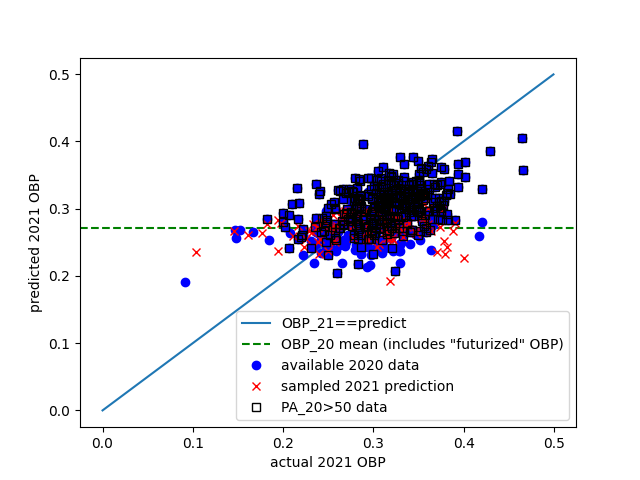
\includegraphics[width=15cm]{code/results.png}
    \caption{Comparison of the predicted OBP vs. the actual OBP. Sampled predictions are plotted separately from the fully modeled predictions.}
    \label{fig:results}
\end{figure}



\bibliographystyle{plain}
\bibliography{refs}

%----------------------------------------------------------------------------------------

\end{document}
